\documentclass[12pt, titlepage]{article}

\usepackage{booktabs}
\usepackage{tabularx}
\usepackage{hyperref}
\hypersetup{
    colorlinks,
    citecolor=black,
    filecolor=black,
    linkcolor=red,
    urlcolor=blue
}
\usepackage[round]{natbib}

%% Comments

%\usepackage{color}
\usepackage[dvipsnames]{xcolor}

\newif\ifcomments\commentstrue

\ifcomments
\newcommand{\authornote}[3]{\textcolor{#1}{[#3 ---#2]}}
\newcommand{\todo}[1]{\textcolor{red}{[TODO: #1]}}
\else
\newcommand{\authornote}[3]{}
\newcommand{\todo}[1]{}
\fi

\newcommand{\wss}[1]{\authornote{blue}{SS}{#1}}
\newcommand{\an}[1]{\authornote{magenta}{Author}{#1}}
\newcommand{\meow}[1]{\authornote{Orchid}{JG}{#1}}

%% Common Parts

\newcommand{\progname}{Kaplan}


% jen things
\usepackage{xr} % reference external documents
\externaldocument{../../Design/MIS/MIS}
\externaldocument{../../Design/MG/MG}
\usepackage{graphicx} % for figures
\usepackage{float} % for H when placing figures
\usepackage{listings} % for code lstlisting
\usepackage{multirow} % for multirow in tables

\begin{document}

\title{Project Title: Unit Verification and Validation Plan for \progname{}} 
\author{Jen  Garner}
\date{\today}
	
\maketitle

\pagenumbering{roman}

\section{Revision History}

\begin{tabularx}{\textwidth}{p{3cm}p{2cm}X}
\toprule {\bf Date} & {\bf Version} & {\bf Notes}\\
\midrule
December 3rd, 2018 (Monday) & 1.0 & First draft \\
\bottomrule
\end{tabularx}

~\newpage

\tableofcontents

\listoftables

\wss{Do not include if not relevant}

\listoffigures

\wss{Do not include if not relevant}

\newpage

\section{Symbols, Abbreviations and Acronyms}

\renewcommand{\arraystretch}{1.2}
\begin{tabular}{l l} 
  \toprule		
  \textbf{symbol} & \textbf{description}\\
  \midrule 
  T & Test\\
  \bottomrule
\end{tabular}\\

\wss{symbols, abbreviations or acronyms -- you can reference the SRS, MG or MIS
  tables if needed}

\newpage

\pagenumbering{arabic}

This document ... \wss{provide an introductory blurb and roadmap of the
  unit V\&V plan}

\section{General Information}

\subsection{Purpose}

This document will identify what testing is going to be done on \progname{}. 
This document is different from the System VnV Plan in that it considers each 
module as already written according to the Module Instance Specification (MIS) 
document. Since each function, method, class, and algorithm has been given, 
they can be tested using a white box approach, where the inputs, outputs, and 
transitions between the inputs and outputs are known.

\wss{Identify software that is being unit tested (verified).}

\subsection{Scope}

The Hardware-Hiding module will not be covered in this unit testing plan, since 
the developer does not have any means or the expertise needed to properly test 
such a module. As mentioned in the System VnV Plan, the energy, geometry, and 
RMSD modules will be tested by running the tests for the libraries that these 
modules import.

The most important modules to test are the two input modules: Molecule Input 
and GA Input. Since this program is likely to be run on a server with multiple 
iterations of different molecules, checking of the inputs before submission is 
very important. If the errors in setup are caught early, jobs (that cannot 
actually run) can be prevented from sitting in queues on the high-performance 
computing (HPC) clusters.

It will be important to test the Crossover \& Mutation (mutations) module, 
since this is how the solutions will evolve over time. If the new population 
members are not correctly initialized (or if they are copies of the old 
population members without any mutation), then the optimization will not work 
and running the program would have been a waste of resources and time.

The GA Input module (gac) is probably the least important module to test, since 
it is only running other modules in a sequence. Basic tests, such as: 1. was 
the Ring initialized, 2. did the Ring change as a result of running the gac 
module, 3. were the outputs and inputs called, can be done on gac if necessary.

Other modules that will be tested include: fitg, tournament, ring, pmem, and 
output.

\wss{What modules are outside of the scope.  If there are modules that are
  developed by someone else, then you would say here if you aren't planning on
  verifying them.  There may also be modules that are part of your software, but
  have a lower priority for verification than others.  If this is the case,
  explain your rationale for the ranking of module importance.}

\section{Plan}
	
\subsection{Verification and Validation Team}

Mulder, c'est moi.

\subsection{Automated Testing and Verification Tools}

The Ayers' Lab group has a linter called Cardboardlint 
\url{https://github.com/theochem/cardboardlint}. If time permits, this linter 
can be joined with Travis CI (Continuous Integration) to enable static code 
checking (for PEP8) and code coverage. Prior to enabling this linter, the 
following libraries can be added to the Travis build:

\begin{itemize}
	\item coverage
	\item pylint
	\item nosetests (also called nose)
	\item pycodestyle
	\item pydocstyle (with numpy convention)
\end{itemize}

The report generated by Travis CI will be uploaded to the VnV Report. The 
.travis.yml file will be added to the \progname{} repository so the 
installation and verification process can be monitored. Eventually the program 
will be made into a conda package itself, then a conda environment can be used 
for an easy installation process.

\wss{What tools are you using for automated testing.  Likely a unit testing
  framework and maybe a profiling tool, like ValGrind.  Other possible tools
  include a static analyzer, make, continuous integration tools, test coverage
  tools, etc.  Explain your plans for summarizing code coverage metrics.}

\subsection{Non-Testing Based Verification}

Some jupyter notebooks (\url{http://jupyter.org/}) will be made by the 
developer as a way to test the geometry module and the energy module. These 
notebooks are an easy way to ensure that the imported libraries behave as 
intended with the \progname{} code and that the developer has correctly 
interpreted the other libraries' documentation and usage. These notebooks will 
be helpful later-on as documentation, in case the user wants to manipulate the 
energy calculations and/or the parts of the geometry that are optimized.

There will be a code review with lab members Kumru Dikmenli and Xiaomin Huang 
during a weekly meeting. Once the SRS has been updated to address comments from 
Prof. Paul Ayers (supervisor), there will also be a code walk-through with the 
supervisor.

\wss{List any approaches like code inspection, code walkthrough, symbolic
  execution etc.  Enter not applicable if you do not plan on any non-testing
  based verification.}

\section{Unit Test Description}

\begin{figure}[H]
	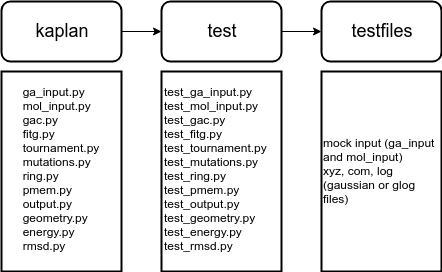
\includegraphics[width=\textwidth]{directory-structure.png}
	\caption{The directory structure for the unit testing. An arrow from A to B 
		implies that B is a subdirectory of A.}
	\label{fig-dir-struct}
\end{figure}

The directory structure for testing is as follows (see Figure 
\ref{fig-dir-struct}). First we have the \textit{kaplan} directory that 
contains the code. Within this directory, there is the \textit{test} 
subdirectory. This \textit{test} directory has a test file (.py) for each 
module. Within the \textit{test} directory there is a \textit{testfiles} 
subdirectory, which contains mostly molecule input and output, as well as 
kaplan-formatted input for the two input modules. Each test file has the naming 
convention: test\_module\_name.py and each function within each of the test 
files has the naming convention: test\_function\_name.py. If the test is for a 
class, then the naming convention for the test becomes: 
test\_Classname\_methodname.py.

\meow{I wasn't sure where to put the above information. It seems relevant to my 
	documentation. Also, I think the naming convention is actually required by 
	nosetests, but I could be wrong.}

\wss{Reference your MIS and explain your overall philosophy for test case
  selection.}

\subsection{Tests for Functional Requirements}

For many of these tests, the numpy python library testing module will be 
utilized. Within that testing module, there is an assert\_raises function. This 
function is used to ensure that the correct errors are raised for a given 
function call and function inputs.

\wss{Most of the verification will be through automated unit testing.  If
  appropriate specific modules can be verified by a non-testing based
  technique.  That can also be documented in this section.}

\subsubsection{GA Input Module} \label{test-ga_input}

\meow{I couldn't figure out how to make the mref work in this document, even 
	when the MG was added as an external document in the tex file. Any 
	suggestions?}

From Section \ref{section-ga_input} in the MIS, we have a set of unit tests for 
the GA Input Module. The purpose of these tests is to ensure that an error is 
raised if the user does one of the following:
\begin{enumerate}
	\item Provides a file name that does not exist in the given directory.
	\item Forgets to include an input parameter or misspells an input parameter.
	\item Puts the same input parameter twice or adds too many input parameters.
	\item Provides input values that do not satisfy the program constraints 
	(for example, num\_slots $<$ num\_filled).
	\item Provides input values of the wrong type (for example, num\_mevs is 
	equal to 3.2, which doesn't make physical sense).
\end{enumerate}
The tests should also confirm that correct input can pass without raising 
errors. A couple of valid and invalid input files will be available in the 
testfiles directory (see Figure \ref{fig-dir-struct}). The valid input files 
can also act as example input for instructional purposes.

\meow{I might need to add a test to see what happens when the user tries to 
open a file that they do not have read permissions for. However, I can't think 
of a reasonable case where this would happen. I'm also not sure how to create 
that error without trying to access someone else's files... I'll assume the 
interpreter error message will be sufficient.}

As per the MIS (Section \ref{section-ga_input}), there are two functions within 
the ga\_input module: read\_ga\_input, which checks the number of inputs and 
ensures the file can be opened (file exists), and verify\_ga\_input, which 
checks that all of the input parameters have been given and that their values 
are of the right type and within the necessary bounds.

\wss{Include a blurb here to explain why the subsections below cover the module.
  References to the MIS would be good.  You will want tests from a black box
  perspective and from a white box perspective.  Explain to the reader how the
  tests were selected.}

\begin{enumerate}

\item{test\_read\_ga\_input\\}

Type: automatic
					
Initial State: None
					
Input: 

\begin{table}[H]
	\begin{tabular}{ccp{4cm}}
		\toprule
		file name & error raised & test covered \\
		\midrule
		example\_ga\_input\_file.txt & None & good input does not raise an 
		error \\
		example2\_ga\_input\_file.txt & None & good input can have extra 
		whitespace and is impervious to capitalization \\
		no-such-file & FileNotFoundError & file does not exist and therefore 
		cannot (and should not) be opened \\
		bad1\_ga\_input\_file.txt & ValueError & num\_mevs appears twice (too 
		many input parameters) \\
		bad2\_ga\_input\_file.txt & ValueError & num\_atoms is not in the input 
		file (missing input parameter) \\
	\end{tabular}
\end{table}
					
Output: None

Test Case Derivation: None

How test will be performed: If the read\_ga\_input function can be called with 
the good input files without raising an error, then the test is assumed to 
pass. Conversely, if the bad inputs raise the expected error as per the 
assert\_raises function, then the test will pass.
					
\item{test\_verify\_ga\_input\\}

Type: automatic
					
Initial State: None
					
Input:

\begin{table}[H]
	\begin{tabularx}{\textwidth}{p{5cm}p{3cm}p{6.5cm}}
		\toprule
		file name or & \multirow{2}{*}{error raised} & \multirow{2}{*}{test 
		covered} \\
		change in ga\_input\_dict*& & \\
		\midrule
		example\_ga\_input\_file.txt & None & good input does not raise an 
		error \\
		example2\_ga\_input\_file.txt & None & good input can have extra 
		whitespace and is impervious to capitalization \\
		bad3\_ga\_input\_file.txt & ValueError & num\_geoms is spelt wrong 
		(input file does not contain all of the expected parameters) \\
		num\_slots = -1 & AssertionError & num\_slots must be positive \\
		num\_filled = 150 & AssertionError & num\_filled must be $\leq$ 
		num\_slots \\
		num\_mevs = -300 & AssertionError & num\_mevs must be positive \\
		num\_swaps = 20 & AssertionError & num\_swaps must be $\leq$ num\_geoms 
		\\
		num\_muts = 30 & AssertionError & num\_muts must be $\leq$ num\_atoms-3 
		\\
		num\_geoms = -2 & AssertionError & num\_geoms must be positive \\
		num\_atoms = 2 & AssertionError & num\_atoms must be $\geq$ 4 \\
		fit\_form = 1 & AssertionError & fit\_form will only be implemented 
		with one function initially; only fit\_form = 0 is accepted \\
		pmem\_dist = 57 & AssertionError & pmem\_dist has to be $\leq$ 
		1/2*num\_slots (rounded down) \\
		coef\_energy = -5 & AssertionError & coef\_energy must be positive \\
		coef\_rmsd = -5 & AssertionError & coef\_rmsd must be positive \\
		t\_size = 25 & AssertionError & t\_size must be $\leq$ num\_filled \\
	\end{tabularx}
\end{table}

\noindent * for changes to the ga\_input\_dict, the other parameters are based 
on the contents of the example\_ga\_input\_file.txt, where we have:
\begin{lstlisting}[language=python, showstringspaces=false]
ga_input_dict = {`num_mevs': `1000', `num_slots': `100',
		 `num_filled': `20', `num_geoms': `3',
		 `num_atoms': `10', `t_size': `7',
		 `num_muts': `3', `num_swaps': `1',
		 `pmem_dist': `5', `fit_form': `0',
		 `coef_energy': `0.5', `coef_rmsd': `0.5'}
\end{lstlisting}
					
Output: None

Test Case Derivation: None

How test will be performed: as with the tests for read\_ga\_input, these tests 
will use the numpy.testing assert\_raises function to ensure that the correct 
errors are raised. The verify\_ga\_input function is also responsible for 
checking the types of the input; if a value (for example, num\_geoms) is 
supposed to be an integer and python cannot convert the input to an integer, 
then an error will be raised. This is not covered by the unit tests, since it 
is assumed that trying to use incorrect types (a string as an integer) will 
yield an obvious error.
    
\end{enumerate}

\subsubsection{Molecule Input Module}

The mol\_input module will be tested in a similar fashion to the 
ga\_input\_module (Section \ref{test-ga_input}), with the added tests as needed 
to check the input geometry, QCM, and BS. As per the module uses hierarchy in 
the module guide document, the mol\_input module uses the geometry and energy 
modules. Therefore, to test this module properly, both of these other modules 
must be adequately tested as well.

\wss{Include a blurb here to explain why the subsections below cover the module.
	References to the MIS would be good.  You will want tests from a black box
	perspective and from a white box perspective.  Explain to the reader how the
	tests were selected.}

\begin{enumerate}
	
\item{test\_read\_mol\_input\\}

Type: automatic

Initial State: None

Input: 
	
\begin{table}[H]
	\begin{tabular}{ccp{4cm}}
		\toprule
		file name & error raised & test covered \\
		\midrule
		example\_mol\_input\_file.txt & None & good input does not raise an 
		error \\
		example2\_mol\_input\_file.txt & None & good input can have extra 
		whitespace and is impervious to capitalization \\
		no-such-file & FileNotFoundError & file does not exist and therefore 
		cannot (and should not) be opened \\
		bad1\_mol\_input\_file.txt & ValueError & qcm appears twice (too 
		many input parameters) \\
		bad2\_mol\_input\_file.txt & ValueError & struct\_type is not in the 
		input file (missing input parameter) \\
	\end{tabular}
\end{table}
	
Output: None

Test Case Derivation: None

How test will be performed: numpy.testing.assert\_raises.

\item{test\_verify\_mol\_input\\}

Type: automatic

Initial State: None

Input:

\begin{table}[H]
	\begin{tabularx}{\textwidth}{p{5cm}p{3cm}p{6.5cm}}
		\toprule
		file name or & \multirow{2}{*}{error raised} & \multirow{2}{*}{test 
			covered} \\
		change in mol\_input\_dict*& & \\
		\midrule
		example\_mol\_input\_file.txt & None & good input does not raise an 
		error \\
		example2\_mol\_input\_file.txt & None & good input can have extra 
		whitespace and is impervious to capitalization \\
		bad3\_mol\_input\_file.txt & ValueError & struct\_input is spelt wrong 
		(input file does not contain all of the expected parameters) \\
		qcm = ``not-a-method" & ValueError & qcm must be available in the 
		chosen program \\
		basis = ``not-a-basis" & ValueError & basis must be available in the 
		chosen program \\
		struct\_input = ``very-bad-smiles-string" & ValueError & SMILES string 
		must be valid \\
		struct\_type = ``not-an-option" & AssertionError & struct\_type must be 
		one of: ``com", ``glog", ``xyz", ``smiles", ``name", or ``cid" \\
		prog = ``unavailable-prog" & AssertionError & prog must equal ``psi4" \\
		charge = ``0.34" & ValueError & charge must be an integer \\
		multip = -2 & AssertionError & multiplicity must be $\geq$ 0 \\
	\end{tabularx}
\end{table}

\noindent * for changes to the mol\_input\_dict, the other parameters are based 
on the contents of the example\_mol\_input\_file.txt, where we have:
\begin{lstlisting}[language=python, showstringspaces=false]
mol_input_dict = {`qcm': `hf', `basis': `sto-3g',
                  `struct_input': `c=cc=c',
                  `struct_type': `smiles', `prog': `psi4',
                  `charge': `0', `multip': `1'}
\end{lstlisting}

Output: None

Test Case Derivation: None

How test will be performed: numpy.testing.assert\_raises.
	
\end{enumerate}

\subsubsection{GA Control Module}

\wss{Include a blurb here to explain why the subsections below cover the module.
	References to the MIS would be good.  You will want tests from a black box
	perspective and from a white box perspective.  Explain to the reader how the
	tests were selected.}

\begin{enumerate}
	
	\item{test-id1\\}
	
	Type: \wss{Functional, Dynamic, Manual, Automatic, Static etc. Most will
		be automatic}
	
	Initial State: 
	
	Input: 
	
	Output: \wss{The expected result for the given inputs}
	
	Test Case Derivation: \wss{Justify the expected value given in the Output 
	field}
	
	How test will be performed: 
	
	\item{test-id2\\}
	
	Type: \wss{Functional, Dynamic, Manual, Automatic, Static etc. Most will
		be automatic}
	
	Initial State: 
	
	Input: 
	
	Output: \wss{The expected result for the given inputs}
	
	Test Case Derivation: \wss{Justify the expected value given in the Output 
	field}
	
	How test will be performed: 
	
	\item{...\\}
	
\end{enumerate}

\subsubsection{Module 1}

\wss{Include a blurb here to explain why the subsections below cover the module.
	References to the MIS would be good.  You will want tests from a black box
	perspective and from a white box perspective.  Explain to the reader how the
	tests were selected.}

\begin{enumerate}
	
	\item{test-id1\\}
	
	Type: \wss{Functional, Dynamic, Manual, Automatic, Static etc. Most will
		be automatic}
	
	Initial State: 
	
	Input: 
	
	Output: \wss{The expected result for the given inputs}
	
	Test Case Derivation: \wss{Justify the expected value given in the Output 
	field}
	
	How test will be performed: 
	
	\item{test-id2\\}
	
	Type: \wss{Functional, Dynamic, Manual, Automatic, Static etc. Most will
		be automatic}
	
	Initial State: 
	
	Input: 
	
	Output: \wss{The expected result for the given inputs}
	
	Test Case Derivation: \wss{Justify the expected value given in the Output 
	field}
	
	How test will be performed: 
	
	\item{...\\}
	
\end{enumerate}

\subsubsection{Module 1}

\wss{Include a blurb here to explain why the subsections below cover the module.
	References to the MIS would be good.  You will want tests from a black box
	perspective and from a white box perspective.  Explain to the reader how the
	tests were selected.}

\begin{enumerate}
	
	\item{test-id1\\}
	
	Type: \wss{Functional, Dynamic, Manual, Automatic, Static etc. Most will
		be automatic}
	
	Initial State: 
	
	Input: 
	
	Output: \wss{The expected result for the given inputs}
	
	Test Case Derivation: \wss{Justify the expected value given in the Output 
	field}
	
	How test will be performed: 
	
	\item{test-id2\\}
	
	Type: \wss{Functional, Dynamic, Manual, Automatic, Static etc. Most will
		be automatic}
	
	Initial State: 
	
	Input: 
	
	Output: \wss{The expected result for the given inputs}
	
	Test Case Derivation: \wss{Justify the expected value given in the Output 
	field}
	
	How test will be performed: 
	
	\item{...\\}
	
\end{enumerate}

\subsubsection{Module 1}

\wss{Include a blurb here to explain why the subsections below cover the module.
	References to the MIS would be good.  You will want tests from a black box
	perspective and from a white box perspective.  Explain to the reader how the
	tests were selected.}

\begin{enumerate}
	
	\item{test-id1\\}
	
	Type: \wss{Functional, Dynamic, Manual, Automatic, Static etc. Most will
		be automatic}
	
	Initial State: 
	
	Input: 
	
	Output: \wss{The expected result for the given inputs}
	
	Test Case Derivation: \wss{Justify the expected value given in the Output 
	field}
	
	How test will be performed: 
	
	\item{test-id2\\}
	
	Type: \wss{Functional, Dynamic, Manual, Automatic, Static etc. Most will
		be automatic}
	
	Initial State: 
	
	Input: 
	
	Output: \wss{The expected result for the given inputs}
	
	Test Case Derivation: \wss{Justify the expected value given in the Output 
	field}
	
	How test will be performed: 
	
	\item{...\\}
	
\end{enumerate}

\subsubsection{Module 1}

\wss{Include a blurb here to explain why the subsections below cover the module.
	References to the MIS would be good.  You will want tests from a black box
	perspective and from a white box perspective.  Explain to the reader how the
	tests were selected.}

\begin{enumerate}
	
	\item{test-id1\\}
	
	Type: \wss{Functional, Dynamic, Manual, Automatic, Static etc. Most will
		be automatic}
	
	Initial State: 
	
	Input: 
	
	Output: \wss{The expected result for the given inputs}
	
	Test Case Derivation: \wss{Justify the expected value given in the Output 
	field}
	
	How test will be performed: 
	
	\item{test-id2\\}
	
	Type: \wss{Functional, Dynamic, Manual, Automatic, Static etc. Most will
		be automatic}
	
	Initial State: 
	
	Input: 
	
	Output: \wss{The expected result for the given inputs}
	
	Test Case Derivation: \wss{Justify the expected value given in the Output 
	field}
	
	How test will be performed: 
	
	\item{...\\}
	
\end{enumerate}

\subsubsection{Module 1}

\wss{Include a blurb here to explain why the subsections below cover the module.
	References to the MIS would be good.  You will want tests from a black box
	perspective and from a white box perspective.  Explain to the reader how the
	tests were selected.}

\begin{enumerate}
	
	\item{test-id1\\}
	
	Type: \wss{Functional, Dynamic, Manual, Automatic, Static etc. Most will
		be automatic}
	
	Initial State: 
	
	Input: 
	
	Output: \wss{The expected result for the given inputs}
	
	Test Case Derivation: \wss{Justify the expected value given in the Output 
	field}
	
	How test will be performed: 
	
	\item{test-id2\\}
	
	Type: \wss{Functional, Dynamic, Manual, Automatic, Static etc. Most will
		be automatic}
	
	Initial State: 
	
	Input: 
	
	Output: \wss{The expected result for the given inputs}
	
	Test Case Derivation: \wss{Justify the expected value given in the Output 
	field}
	
	How test will be performed: 
	
	\item{...\\}
	
\end{enumerate}

\subsubsection{Module 1}

\wss{Include a blurb here to explain why the subsections below cover the module.
	References to the MIS would be good.  You will want tests from a black box
	perspective and from a white box perspective.  Explain to the reader how the
	tests were selected.}

\begin{enumerate}
	
	\item{test-id1\\}
	
	Type: \wss{Functional, Dynamic, Manual, Automatic, Static etc. Most will
		be automatic}
	
	Initial State: 
	
	Input: 
	
	Output: \wss{The expected result for the given inputs}
	
	Test Case Derivation: \wss{Justify the expected value given in the Output 
	field}
	
	How test will be performed: 
	
	\item{test-id2\\}
	
	Type: \wss{Functional, Dynamic, Manual, Automatic, Static etc. Most will
		be automatic}
	
	Initial State: 
	
	Input: 
	
	Output: \wss{The expected result for the given inputs}
	
	Test Case Derivation: \wss{Justify the expected value given in the Output 
	field}
	
	How test will be performed: 
	
	\item{...\\}
	
\end{enumerate}

\subsubsection{Module 1}

\wss{Include a blurb here to explain why the subsections below cover the module.
	References to the MIS would be good.  You will want tests from a black box
	perspective and from a white box perspective.  Explain to the reader how the
	tests were selected.}

\begin{enumerate}
	
	\item{test-id1\\}
	
	Type: \wss{Functional, Dynamic, Manual, Automatic, Static etc. Most will
		be automatic}
	
	Initial State: 
	
	Input: 
	
	Output: \wss{The expected result for the given inputs}
	
	Test Case Derivation: \wss{Justify the expected value given in the Output 
	field}
	
	How test will be performed: 
	
	\item{test-id2\\}
	
	Type: \wss{Functional, Dynamic, Manual, Automatic, Static etc. Most will
		be automatic}
	
	Initial State: 
	
	Input: 
	
	Output: \wss{The expected result for the given inputs}
	
	Test Case Derivation: \wss{Justify the expected value given in the Output 
	field}
	
	How test will be performed: 
	
	\item{...\\}
	
\end{enumerate}

\subsubsection{Module 1}

\wss{Include a blurb here to explain why the subsections below cover the module.
	References to the MIS would be good.  You will want tests from a black box
	perspective and from a white box perspective.  Explain to the reader how the
	tests were selected.}

\begin{enumerate}
	
	\item{test-id1\\}
	
	Type: \wss{Functional, Dynamic, Manual, Automatic, Static etc. Most will
		be automatic}
	
	Initial State: 
	
	Input: 
	
	Output: \wss{The expected result for the given inputs}
	
	Test Case Derivation: \wss{Justify the expected value given in the Output 
	field}
	
	How test will be performed: 
	
	\item{test-id2\\}
	
	Type: \wss{Functional, Dynamic, Manual, Automatic, Static etc. Most will
		be automatic}
	
	Initial State: 
	
	Input: 
	
	Output: \wss{The expected result for the given inputs}
	
	Test Case Derivation: \wss{Justify the expected value given in the Output 
	field}
	
	How test will be performed: 
	
	\item{...\\}
	
\end{enumerate}

\subsubsection{Module 1}

\wss{Include a blurb here to explain why the subsections below cover the module.
	References to the MIS would be good.  You will want tests from a black box
	perspective and from a white box perspective.  Explain to the reader how the
	tests were selected.}

\begin{enumerate}
	
	\item{test-id1\\}
	
	Type: \wss{Functional, Dynamic, Manual, Automatic, Static etc. Most will
		be automatic}
	
	Initial State: 
	
	Input: 
	
	Output: \wss{The expected result for the given inputs}
	
	Test Case Derivation: \wss{Justify the expected value given in the Output 
	field}
	
	How test will be performed: 
	
	\item{test-id2\\}
	
	Type: \wss{Functional, Dynamic, Manual, Automatic, Static etc. Most will
		be automatic}
	
	Initial State: 
	
	Input: 
	
	Output: \wss{The expected result for the given inputs}
	
	Test Case Derivation: \wss{Justify the expected value given in the Output 
	field}
	
	How test will be performed: 
	
	\item{...\\}
	
\end{enumerate}

\subsection{Tests for Nonfunctional Requirements}

\wss{If there is a module that needs to be independently assessed for
  performance, those test cases can go here.  In some projects, planning for
  nonfunctional tests of units will not be that relevant.}

\wss{These tests may involve collecting performance data from previously
  mentioned functional tests.}

\subsubsection{Module ?}
		
\begin{enumerate}

\item{test-id1\\}

Type: \wss{Functional, Dynamic, Manual, Automatic, Static etc. Most will
  be automatic}
					
Initial State: 
					
Input/Condition: 
					
Output/Result: 
					
How test will be performed: 
					
\item{test-id2\\}

Type: Functional, Dynamic, Manual, Static etc.
					
Initial State: 
					
Input: 
					
Output: 
					
How test will be performed: 

\end{enumerate}

\subsubsection{Module ?}

...

\subsection{Traceability Between Test Cases and Modules}

\wss{Provide evidence that all of the modules have been considered.}

\bibliographystyle{plainnat}

\bibliography{SRS}

\newpage

\section{Appendix}

\wss{This is where you can place additional information, as appropriate}

\subsection{Symbolic Parameters}

\wss{The definition of the test cases may call for SYMBOLIC\_CONSTANTS.
Their values are defined in this section for easy maintenance.}

\end{document}